\documentclass[11pt]{article}

\usepackage[utf8]{inputenc}
\usepackage[T1]{fontenc}
\usepackage[spanish,es-tabla]{babel}
\usepackage{lmodern}
\usepackage[a4paper,margin=2cm]{geometry}
\usepackage{graphicx}
\usepackage{xcolor}
\usepackage{colortbl}
\usepackage{array}
\usepackage{enumitem}
\usepackage{tikz}
\usetikzlibrary{backgrounds}
\usepackage[hidelinks]{hyperref}

\graphicspath{{capturas/}}
\setlength{\parskip}{0.5em}
\setlength{\parindent}{0pt}
\renewcommand{\arraystretch}{1.35}
\setlist{nosep,leftmargin=1.2em}

\definecolor{marca}{HTML}{0B3A5C}
\definecolor{borde}{HTML}{B8C4CE}
\definecolor{barra}{HTML}{E6ECF1}
\definecolor{telefono}{HTML}{1F2933}
\definecolor{suave}{HTML}{F3F6F9}
\arrayrulecolor{borde}

% Captura de escritorio dentro de una ventana de navegador sencilla.
% #1 alto de la imagen, #2 archivo
\newcommand{\escritorio}[2]{%
  \begin{tikzpicture}[baseline=(img.south)]
    \node[inner sep=0] (img) {\includegraphics[height=#1]{#2}};
    \fill[barra] ([yshift=0.42cm]img.north west) rectangle (img.north east);
    \foreach \i/\c in {0/red!55, 1/orange!65, 2/green!50!black!45}
      \fill[\c] ([xshift={0.25cm+\i*0.28cm}, yshift=0.21cm]img.north west) circle (0.07cm);
    \draw[borde, line width=0.8pt, rounded corners=3pt]
      ([yshift=0.42cm]img.north west) rectangle (img.south east);
  \end{tikzpicture}}

% Captura de móvil dentro de un marco de teléfono.
% #1 alto de la imagen, #2 archivo
\newcommand{\movil}[2]{%
  \begin{tikzpicture}[baseline=(img.south)]
    \node[inner sep=0] (img) {\includegraphics[height=#1]{#2}};
    \begin{scope}[on background layer]
      \fill[telefono, rounded corners=9pt]
        ([shift={(-0.14cm,0.3cm)}]img.north west) rectangle ([shift={(0.14cm,-0.3cm)}]img.south east);
    \end{scope}
    \fill[telefono!45] ([yshift=0.15cm]img.north) circle (0.045cm);
  \end{tikzpicture}}

% Ícono del botón de menú (tres líneas).
\newcommand{\iconomenu}{\tikz[baseline=-0.25ex]{\foreach \y in {0,0.085,0.17} \draw[line width=0.7pt, line cap=round] (0,\y) -- (0.25,\y);}}

% Pie corto debajo de cada captura.
\newcommand{\pie}[1]{{\small\color{marca}\textbf{#1}}}

% Recuadro con la lista de cambios de cada pantalla.
\newcommand{\cambios}[1]{%
  \par\smallskip\noindent
  \colorbox{suave}{\begin{minipage}{\dimexpr\linewidth-2\fboxsep\relax}
    \vspace{4pt}\textbf{¿Qué cambia en el celular?}\par\smallskip
    #1\vspace{4pt}
  \end{minipage}}\par}

\title{Diseño responsivo\\[0.3em]
\large Loard - Hito 2 - Módulo II: Arquitectura de frontend y componentización}
\author{}
\date{}

\usepackage{pdfpages}

\begin{document}
\maketitle

\section{Introducción}


Loard se usa en dos lugares muy distintos: en la \textbf{oficina}, desde un computador, y en la \textbf{obra}, desde un celular. Para que funcione bien en los dos casos, desde el diseño se definió una \textbf{retícula}: una cuadrícula invisible de columnas sobre la que se ubica todo el contenido de la pantalla (títulos, tarjetas, tablas y formularios). Es la misma técnica que usan la mayoría de las aplicaciones y páginas web actuales para verse bien en cualquier dispositivo.

La retícula cambia según el ancho de la pantalla. En una pantalla grande hay más columnas y los elementos se ponen uno al lado del otro; en una pequeña hay menos columnas y los elementos se apilan uno debajo del otro.

\begin{center}
\begin{tabular}{|>{\bfseries}m{2.6cm}|m{3.8cm}|>{\centering\arraybackslash}m{2.2cm}|m{5.6cm}|}
\hline
\rowcolor{barra}
\textbf{Dispositivo} & \textbf{Ancho de pantalla} & \textbf{Columnas} & \textbf{Menú principal} \\ \hline
Celular & Menos de 600 px & 4 & Se abre con el botón \iconomenu{}. \\ \hline
Tableta & De 600 a 1023 px & 8 & Se abre con el botón \iconomenu{}. \\ \hline
Computador & Desde 1024 px & 12 & Fijo a la izquierda. \\ \hline
\end{tabular}
\end{center}

\textbf{Todas las pantallas del prototipo se construyen sobre esta misma retícula} y con los mismos componentes compartidos (ver el \emph{Inventario de componentes}). Por eso, cuando cambia el tamaño de la pantalla, cada vista se reorganiza sola y no hay que diseñar una versión aparte para el celular. Es una sola aplicación, con los mismos datos y las mismas acciones; solo cambia la forma en que se acomoda el contenido.

\subsection*{Qué se muestra en este documento}

Las pantallas principales del prototipo en dos tamaños, una al lado de la otra:

\begin{itemize}
  \item \textbf{Escritorio}: pantalla de computador (1440 píxeles de ancho).
  \item \textbf{Móvil}: pantalla de celular (390 píxeles de ancho, el tamaño de un teléfono común).
\end{itemize}

Todas las capturas se tomaron del prototipo en funcionamiento.

\newpage
\section{Pantalla principal: Cortes de obra}

Es la primera pantalla que ve el Ingeniero Residente al entrar. Reúne las cifras del contrato, el buscador y la lista de cortes registrados.

\begin{center}
\begin{tabular}{@{}c@{\hspace{0.7cm}}c@{}}
\escritorio{7.4cm}{cortes-escritorio} & \movil{7.4cm}{cortes-movil-inicio} \\[2pt]
\pie{Escritorio} & \pie{Móvil}
\end{tabular}
\end{center}

Al bajar en el celular, la lista de cortes se convierte en tarjetas y el menú se abre con el botón de las tres líneas:

\begin{center}
\begin{tabular}{@{}>{\centering\arraybackslash}m{4.4cm}@{\hspace{0.6cm}}>{\centering\arraybackslash}m{4.4cm}@{\hspace{0.6cm}}m{6.9cm}@{}}
\movil{8.8cm}{cortes-movil-tarjetas} &
\movil{8.8cm}{cortes-movil-menu} &
\cambios{
\begin{itemize}
  \item \textbf{Menú:} en escritorio está siempre a la izquierda; en el celular se esconde y aparece al tocar el botón \iconomenu{}.
  \item \textbf{Cifras:} las tres tarjetas pasan de estar en una fila a estar una debajo de otra.
  \item \textbf{Lista de cortes:} la tabla se convierte en una tarjeta por corte, con sus datos uno debajo del otro. No hay que mover la pantalla hacia los lados.
  \item \textbf{Botón ``Registrar corte'':} sube debajo del título para tenerlo a mano.
  \item \textbf{Barra superior:} el nombre del contrato se recorta y el rol pasa al menú.
\end{itemize}}
\\[2pt]
\pie{Lista como tarjetas} & \pie{Menú abierto} &
\end{tabular}
\end{center}

\newpage
\section{Personal SST}

Pantalla de Coordinación SST con el estado de cada trabajador. Los trabajadores bloqueados aparecen primero y en rojo.

\begin{center}
\begin{tabular}{@{}c@{\hspace{0.7cm}}c@{}}
\escritorio{7.4cm}{sst-escritorio} & \movil{7.4cm}{sst-movil} \\[2pt]
\pie{Escritorio} & \pie{Móvil}
\end{tabular}
\end{center}

\cambios{
\begin{itemize}
  \item \textbf{Cifras:} las cuatro tarjetas (bloqueados, por vencer y habilitados) se acomodan de a dos por fila.
  \item \textbf{Lista de trabajadores:} cada fila de la tabla se convierte en una tarjeta con nombre, estado, motivo y vencimiento.
  \item \textbf{Lo importante se conserva:} el motivo del bloqueo se sigue leyendo completo, el color rojo de alerta se mantiene y se conserva el orden ``críticos primero''.
  \item \textbf{Botón ``Ver ficha'':} queda dentro de cada tarjeta, grande y fácil de tocar.
\end{itemize}}

\newpage
\section{Registrar corte de obra}

Formulario que llena el residente para reportar lo ejecutado en el periodo. Es la pantalla que más se usa desde la obra.

\begin{center}
\begin{tabular}{@{}c@{\hspace{0.7cm}}c@{}}
\escritorio{7.4cm}{formulario-escritorio} & \movil{7.4cm}{formulario-movil} \\[2pt]
\pie{Escritorio} & \pie{Móvil}
\end{tabular}
\end{center}

\cambios{
\begin{itemize}
  \item \textbf{Una sola columna:} en escritorio las fechas de inicio y fin van lado a lado; en el celular van una debajo de la otra.
  \item \textbf{Campos más grandes:} los campos y botones crecen para poder tocarlos fácilmente con el dedo.
  \item \textbf{Botones a la mano:} ``Guardar corte'' y ``Volver a cortes'' siguen fijos abajo, como en escritorio, pero se ponen uno encima del otro para que quepan completos. Así no hay que bajar hasta el final para guardar.
\end{itemize}}

\newpage
\section{Resumen}

\begin{center}
\begin{tabular}{|>{\bfseries\raggedright\arraybackslash}m{4.2cm}|>{\raggedright\arraybackslash}m{5.7cm}|>{\raggedright\arraybackslash}m{5.7cm}|}
\hline
\rowcolor{barra}
\textbf{Elemento} & \textbf{Escritorio} & \textbf{Móvil} \\ \hline
Menú & Fijo a la izquierda. & Se abre con el botón \iconomenu{}. \\ \hline
Barra superior & Nombre completo del contrato y rol del usuario. & Nombre del contrato recortado; el rol se ve en el menú. \\ \hline
Tarjetas de cifras & Todas en una fila. & Una o dos por fila. \\ \hline
Tablas & Filas y columnas. & Una tarjeta por registro. \\ \hline
Formularios & Centrados, con campos lado a lado. & Una sola columna. \\ \hline
Botones y campos & Tamaño normal para el ratón. & Más grandes, para tocar con el dedo. \\ \hline
Botones del formulario & Fijos abajo, uno al lado del otro. & Fijos abajo, uno encima del otro. \\ \hline
Mover la pantalla hacia los lados & Nunca es necesario. & Nunca es necesario. \\ \hline
\end{tabular}
\end{center}

En resumen, la persona que trabaja en la oficina ve toda la información de un vistazo, y la que está en la obra puede consultar y registrar datos desde su celular sin perder información ni acciones.

% APORTE HU01-HU02-HU07-HU08
\clearpage
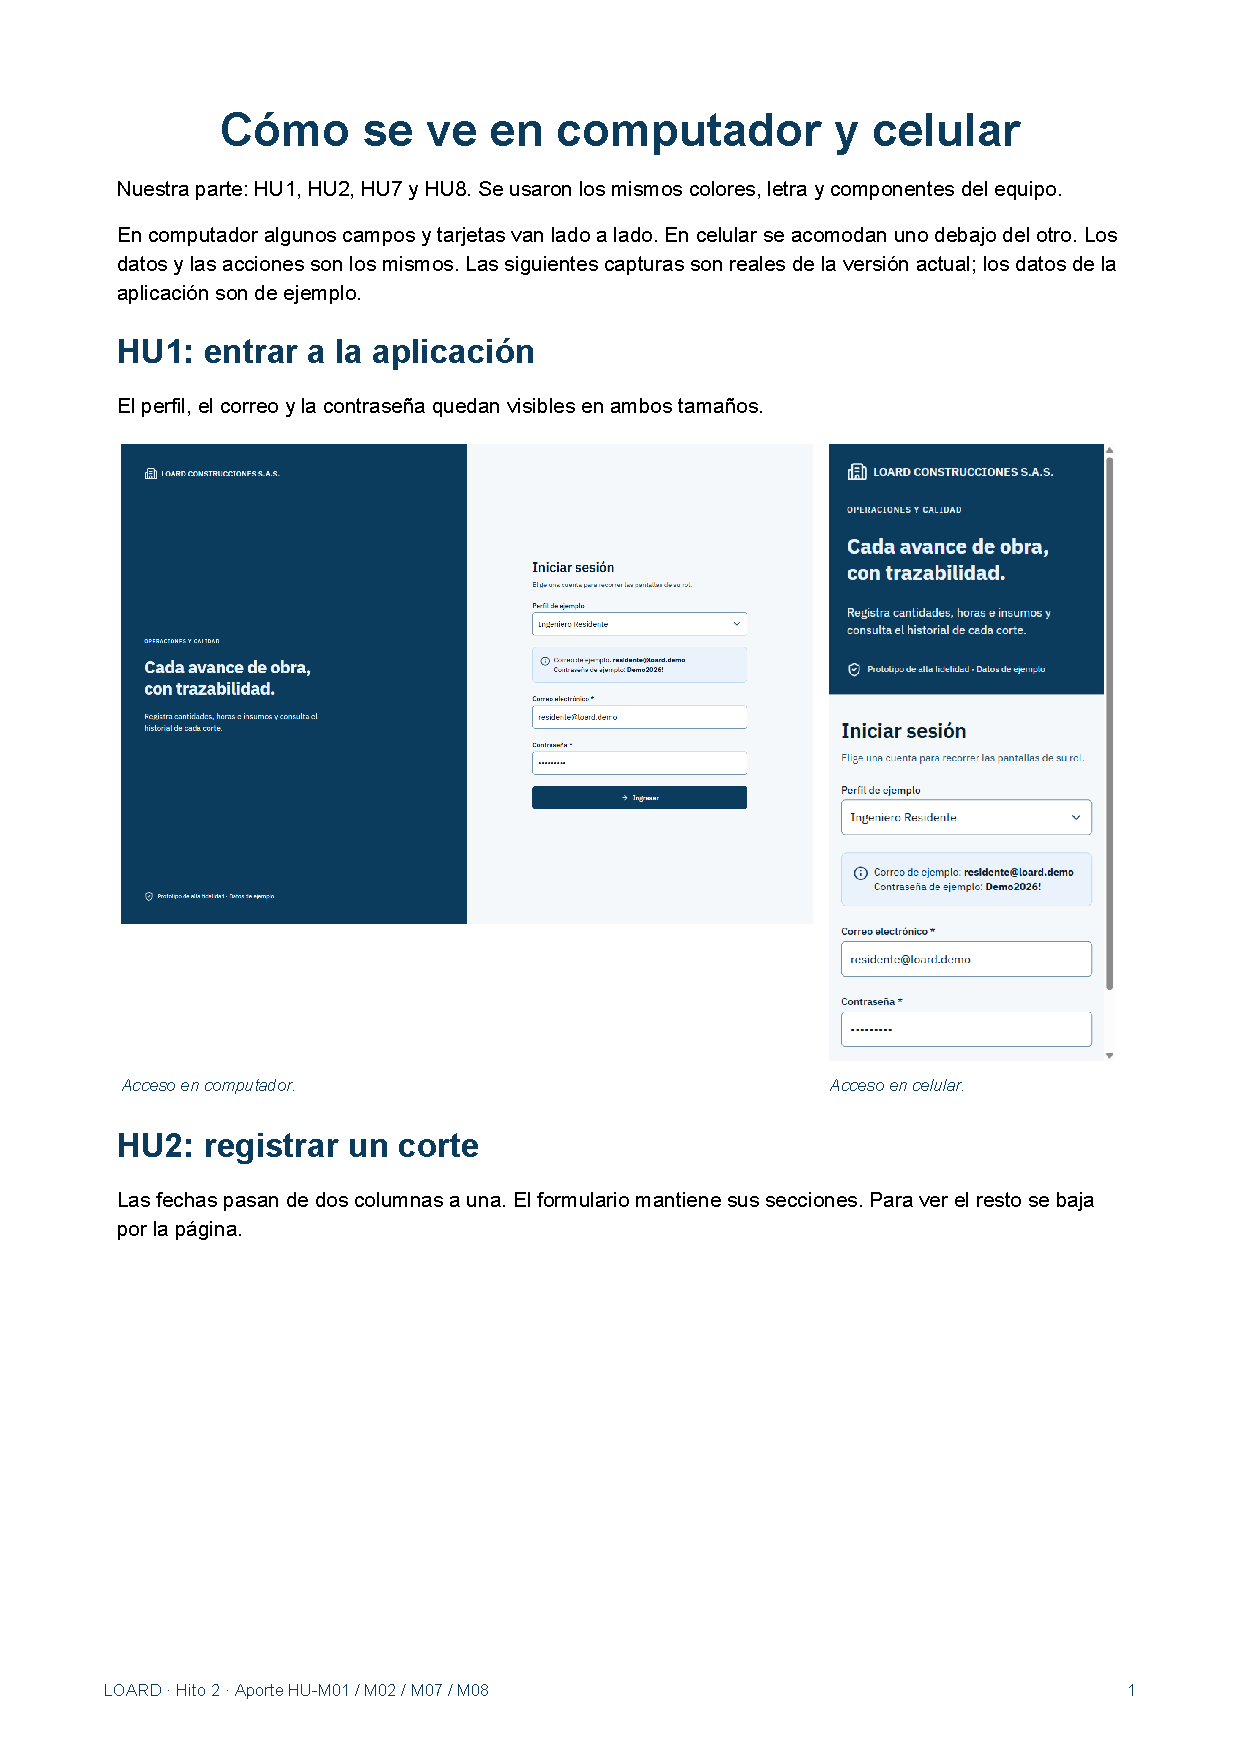
\includepdf[pages=-]{../../Aportes-HU01-HU02-HU07-HU08/02-responsivo.pdf}

\end{document}
